\documentclass[a4paper,english]{report}
    
    \title{Projekt Medieninformatik\\Facial Expresson Recognition\\ Using A State Of The Art CNN}
    \date{WS17/18}
    \author{Lewe Ohlsen\\ Fachhochschule Wedel}
    
    \usepackage[utf8]{inputenc}  
    \usepackage[inline]{enumitem}
    \usepackage{tikz}
    \usepackage{pgfgantt}

    \begin{document}
        \maketitle
        \newpage
            \tableofcontents
        \newpage
        
		        
        
        \section{Introduction}
            Automatically recognizing facial expressions is an interesting and challenging problem in many fields, including human computer interaction (HCI) and artificial emotional intelligence.
            The projects goal is to build a device to process live webcam
            images, detect faces and classify the emotion of each face.
            In order to get started with deep learning techniques and state 
            of the art neural networks, I am participating in a Facial 
            Expression Recognition 
            Challenge\footnote{https://www.kaggle.com/c/challenges-in-representation-learning-facial-expression-recognition-challenge/data} 
            on Kaggle.
            
            As Convolutional Neural Networks (CNNs) have proven to be successful with many kinds of image classification  problems, I will focus on building a classifier using a state of the art CNN implementation.
        \section{Roadmap}
            \begin{ganttchart}{1}{16}
                \gantttitle{Calendar Week}{16} \\
                \gantttitlelist{46,...,52,1,2,3,4,5,6,7,8,9}{1} \\
                
                \ganttbar{MNIST Tutorial}{1}{2} \\
                \ganttlinkedbar{Data preparation}{3}{3} \\
                \ganttbar{implementing a simple linear model}{3}{4} \\                                
                \ganttlinkedbar{implementing a CNN}{4}{10} \\                
                
                %\ganttlinkedbar{Task 2}{3}{7} \ganttnewline
                \ganttmilestone{processing Webcam images}{8} \ganttnewline
                \ganttlinkedbar{Tuning parameters}{10}{12}
                
                %\ganttlink{elem1}{elem2}            
                
            \end{ganttchart}
        \chapter{About the Dataset}
        
        The Dataset consists of 48x48 pixel grayscale images of faces. 
        These images have been centered automatically to show a similar 
        region of the face in every sample. All the images are labeled
        with the visible facial expression according to Ekmans (…) face classification (1970s).
        
        Initially, the dataset is split into two subsets: A training set 
        that is used to fit the prediction and a test set to evaluate the prediction results and compute the generalization error. The generalisation error is the average error for data that the model has never seen (e.g live webcam images).



        \begin{figure}[h]
            \centering
            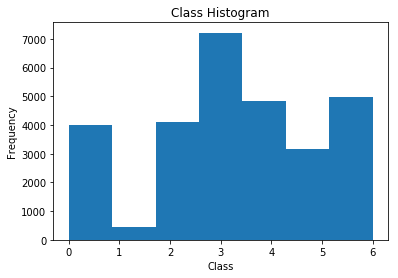
\includegraphics[width=0.6\textwidth]{figures/class_dist.png}
            \caption{Class distribution across the training dataset}
            \label{fig:classdist}
        \end{figure}
        
        
        \chapter{Challenges}
        \section{Recognizing Faces}
        \section{Classifying Facial Expressions}
        \chapter{Feedforward Neural Networks}
        A feedforward neural network can be thought of as a prediction function f(x) = y where x is a fixed-size vector that represents the input data. In this
        case, the image is represented as a 2304-dimensional vector, each component
        being the grayscale intensity of a pixel [0..1]. y is a 7-dimensional vector,
        each component representing the computed probability of the image belonging 
        to a certain class. The function f is actually a computational graph (DAG)…
        
        The flow of information is uni-directional and not cyclic.

        \section{Perceptrons}

        \section{Cost Function}

        \section{Optimizers}
        \section{Gradient Descend}
        \section{Backpropagation}        
        \chapter{Convolutional Neural Networks}
        %\section{Feature Extraction}
        \section{Convolutions}
    	\section{Pooling}
    	Downsampling the image or hidden-layer output matrix and providing an abstracted form of the representation. This allows for assumptions to be made about features contained in the sub-regions of the image.
    	
    	Max-pooling e.g a 2x2 filter running over the image with a stride of 2 and taking the max value for each position.
    	
   		\begin{figure}[h]
    		\centering
    		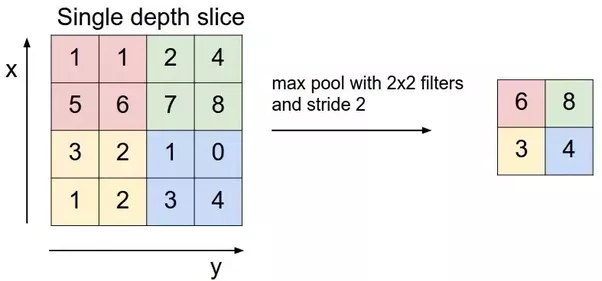
\includegraphics[width=0.6\textwidth]{figures/max_pooling.png}
    		\caption{Max-pooling a 4x4-pixels image with a 2x2 filter and a stride of 2}
    		\label{fig:maxpooling}
    	\end{figure}
    	
    	(Source: Stanford's CS231n github)
    	
        \section{Filters}
        \section{Layers and Dropouts}
        \chapter{Processing Live Images}
    \end{document}
    
    
    
    
    
    
    
    